\documentclass{article}
\usepackage{amsmath}
\title{PHYS 360A/B \\ Experiment 20: Nuclear Magnetic Resonance}
\author{Mikhail Roslikov \and Kamalesh Paluru}
\date{\today}

\usepackage{hyperref}
\usepackage{geometry}
\usepackage{graphicx}
\usepackage{pgfplots}
\usepackage{tikz-3dplot}
\usepackage{tikz}

\tdplotsetmaincoords{60}{115}
\pgfplotsset{compat=newest}

\geometry{
    top=1in,
    bottom=1in
}

\hypersetup{
    colorlinks=true,
    linkcolor=blue,
    filecolor=blue,
    urlcolor=blue,
    citecolor=YellowOrange,
    pdftitle={Nuclear Magnetic Resonance}
}

\newcommand{\degree}{$^{\circ}$ }

\newcommand{\sphere}[2]{
    \begin{tikzpicture}[tdplot_main_coords, scale = 2.5]
        % Create a point (P)
        \coordinate (P) at #1;

        % Line from the origin to (P)
        \draw[thick, -stealth] (0,0,0) -- (P) node[#2] {$\vec{M}$};

        % Draw shaded circle
        \shade[ball color = lightgray,
            opacity = 0.5
        ] (0,0,0) circle (1cm);

        % draw arcs
        \tdplotsetrotatedcoords{0}{0}{0};
        \draw[dashed,
            tdplot_rotated_coords,
            gray
        ] (0,0,0) circle (1);

        % Axes in 3 d coordinate system
        \draw[-stealth] (0,0,0) -- (1.80,0,0)
        node[below left] {$x$};

        \draw[-stealth] (0,0,0) -- (0,1.30,0)
        node[below right] {$y$};

        \draw[-stealth] (0,0,0) -- (0,0,1.30)
        node[above] {$z$};

        \draw[dashed, gray] (0,0,0) -- (-1,0,0);
        \draw[dashed, gray] (0,0,0) -- (0,-1,0);

        % Add small circle at (P)
        \draw[fill = lightgray!50] (P) circle (0.5pt);
    \end{tikzpicture}
}

\begin{document}

\maketitle

\newpage

\tableofcontents

\newpage

\begin{abstract}
    % Your abstract content goes here.
\end{abstract}

\newpage

\section{Introduction}\label{sec:introduction}
% Your introduction content goes here.
Hello World!

\newpage

\section{Theoretical Background}\label{sec:theoretical-background}
% Your theoretical background content goes here.

\newpage

\section{Experimental Design and Procedure}\label{sec:experimental-design-and-procedure}

\newpage

\section{Analysis}\label{sec:analysis}

\subsection{Finding Resonance}\label{subsec:finding-resonance}

\begin{figure}[h]
    \centering
    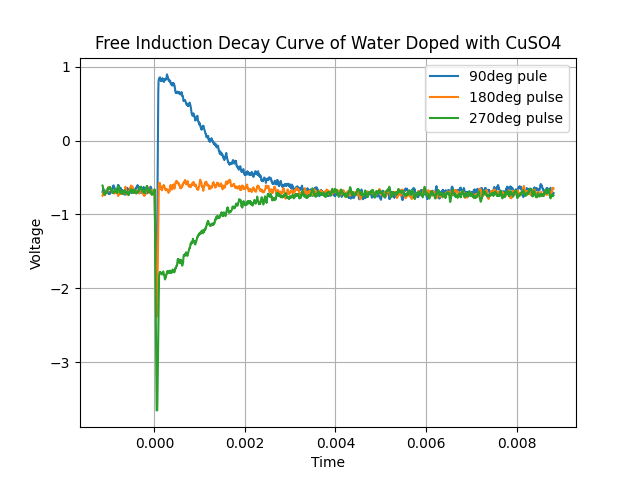
\includegraphics[scale = 0.78]{./images/B1}
    \caption{Free Induction Decay NMR signals for 90$^{\circ}$, 180$^{\circ}$, and 270$^{\circ}$ pulses}
    \label{fig:B1_FID}
\end{figure}

\subsubsection{Voltage at t = 0s}
\textbf{90\degree Pulse}
\begin{itemize}
    \item A 90\degree pulse is a pulse that is applied long enough to tip the magnetization vector by 90\degree from its initial direction (at a small angle with the positive z-axis) in the rotating frame:
    \begin{center}
        \sphere{(0.05, 0, 1)}{right}
        \sphere{(0, 1, 0)}{below}
    \end{center}
    \item Now, nearly half the spins are in the ``up'' state and the other half are in the ``down'' state.
    \item Since $\vec{M}$ is in the x-y plane, the z component of the magnetization vector vanishes:
    \[ M_z = 0 \]
    \item This is a higher energy state than the equilibrium state with the magnetization vector, $\vec{M}$, pointing along the positive z-axis.
    \item The receiver gain was adjusted so that the precessing $\vec{M}$ induced\footnote{According to Faraday's law.} a current in the coil as shown in the 90\degree trace of Figure~\ref{fig:B1_FID}.
\end{itemize}

\textbf{180\degree Pulse}
\begin{itemize}
    \item If we apply the pulse for twice as long (increase the pulse width to twice that of the 90\degree pulse), we rotate the magnetization vector by 180\degree:
    \begin{center}
        \sphere{(0.05, 0, 1)}{right}
        \sphere{(0.05, 0, -1)}{right}
    \end{center}
    \item Most of the spin are now in the ``down'' state.
    \item However, this magnetization vector doesn't induce current in the coils since the component in the x-y plane is nearly 0.
\end{itemize}

\textbf{270\degree Pulse}
\begin{itemize}
    \item This time, the pulse is applied long enough to rotate $\vec{M}$ by an additional 180\degree from the 90\degree case:
    \begin{center}
        \sphere{(0.05, 0, 1)}{right}
        \sphere{(0, -1, 0)}{below}
    \end{center}
    \item That is, $\vec{M}$ returns to the x-y plane but is anti-parallel to $\vec{M}$ in the 90\degree pulse case:
    \[ \vec{M}_{270^\circ} = -\vec{M}_{90^\circ} \]
    \item It hence precesses in the opposite sense of rotation as the 90\degree case\footnote{And vice versa.}.
    \item According to Faraday's law, the direction of the current $\vec{M}_{180^\circ}$ induces in the coil is opposite to that of $\vec{M}_{90^\circ}$.
    \item This is why we see a current that is -$I_{90^\circ}$ induced in the 270\degree case in Figure~\ref{fig:B1_FID}.
\end{itemize}

\subsubsection{Free Induction Decay}
\begin{itemize}
    \item For all three pulses, we see that the signal vanishes over time.
    \item Recall that for the 90\degree and 270\degree pulses, the magnetization vector is in the x-y plane.
    \item Because of small variations in the magnetic field that the magnetic moments, $\vec{\mu}$, for each particle experience, the magnetic moments being to randomly dephase.
    \item They spread out in the x-y plane causing the magnetization vector and hence the induced current to vanish as a whole.
\end{itemize}

\subsection{The Free Induction Decay and $T_2$}\label{subsec:the-free-induction-decay-and-$t_2$}
\begin{itemize}
    \item In this section, we take a closer look at the FID observed in the 90\degree and 270\degree traces of Figure~\ref{fig:B1_FID} (for different samples).
    \item For the same 90\degree pulse, we have the following FID traces:
    \begin{figure}[h]
        \centering
        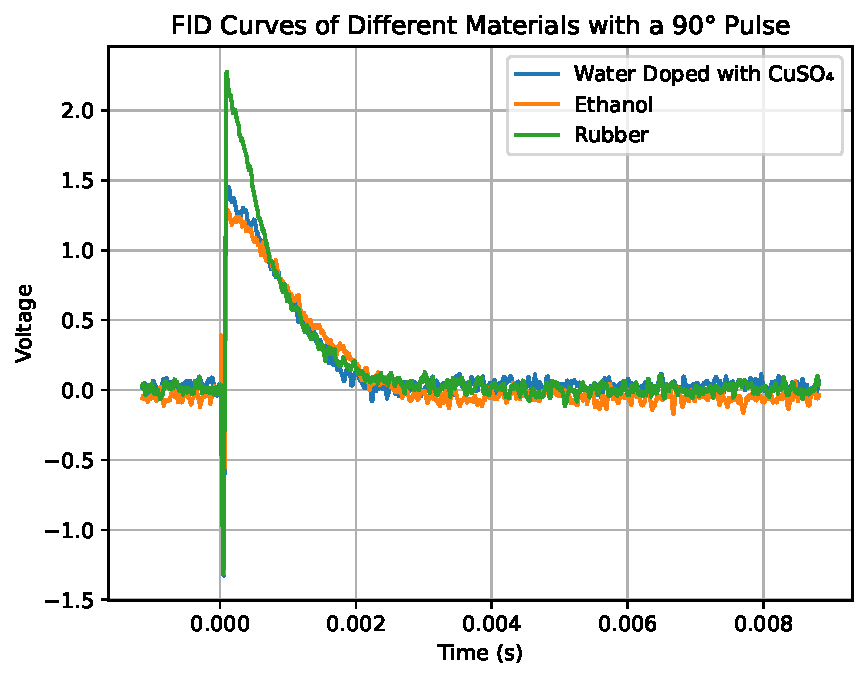
\includegraphics[scale = 0.78]{./images/B2}
        \caption{FID for the 90$^{\circ}$ pulse in water doped with CuSO$_4$, ethanol, and rubber}
        \label{fig:B2_FID}
    \end{figure}
\end{itemize}

\subsubsection{Finding $T_2$}
\textbf{Analytically}
\begin{itemize}
    \item On plotting the traces in Figure~\ref{fig:B2_FID} on a semi-log graph (along with the best fit lines), we get:
    \begin{figure}[h!]
        \centering
        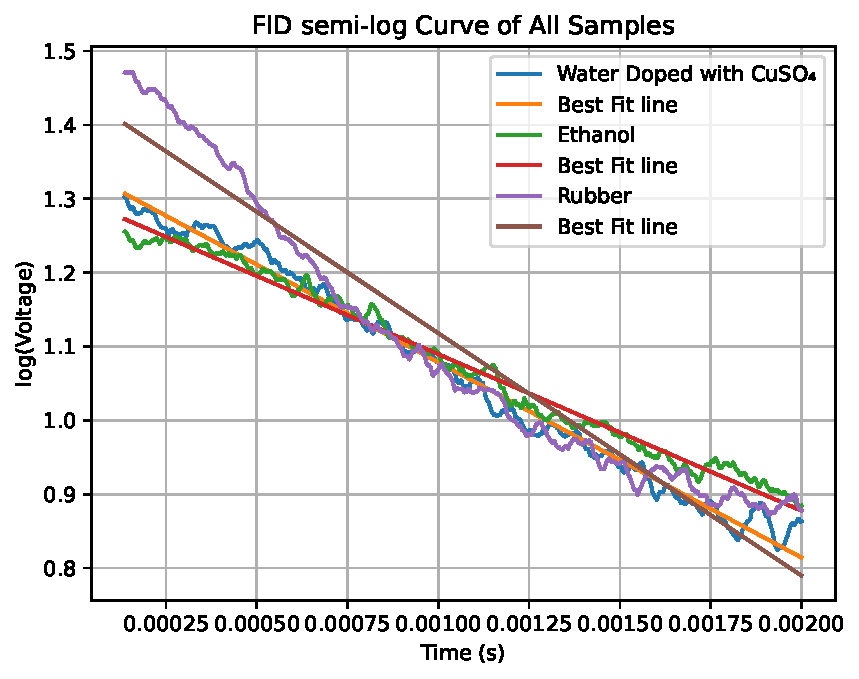
\includegraphics[scale = 0.78]{./images/B2_log_best_fit}
        \caption{$\ln(M_{xy}) = -\frac{t}{T_2^*} + \ln(M_0)$ plotted for the three traces in Figure~\ref{fig:B2_FID}}
        \label{fig:B2_FID_log_best_fit}
    \end{figure}

    \item We can find $T_2^*$ using the following equation:
    \[ M_{xy}(t) = M_0 e^{-\frac{t}{T_2^*}} \]
    Here, $M_{xy}(t)$ is the trace seen in Figure~\ref{fig:B2_FID},\\
    $M_0$ is the magnetization at $t=0$,\\
    $t$ is the time.
    \item We can take the $\ln$ of both sides to get:
    \[ \ln(M_{xy}) = \ln(M_0) + \ln\left(e^{-\frac{t}{T_2^*}}\right) \]
    \[ \ln(M_{xy}) = -\frac{t}{T_2^*} + \ln(M_0) \]
    \item Comparing this to $y = mx + c$, we see that the slope, $m$, is given by:
    \[ m = -\frac{1}{T_2^*} \]
    \[ \implies T_2^* = -\frac{1}{m} \]
\end{itemize}
\textbf{Sample Calculation}
\begin{itemize}
    \item Consider $m = -328.236$s$^{-1}$ for Doped Water in Table~\ref{tab:B2_FID_log_best_fit_table}:
    \[ T_2^* = -\frac{1}{-328.236\text{s}^{-1}} \]
    \[ T_2^* = -\frac{1}{-328.236}\]
    \[ T_2^* = 0.003047\text{s} \]
    \item We can hence find $T_2^*$ from the slopes of the best fit lines in Figure~\ref{fig:B2_FID_log_best_fit} for the other samples:
    \begin{table}[h]
        \centering
        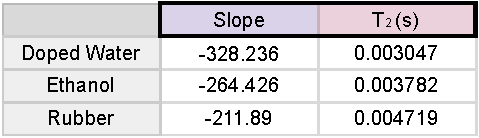
\includegraphics[scale = 0.78]{./images/B2_T2-crop}
        \caption{Slopes of best fit lines and calculated $T_2^*$}
        \label{tab:B2_FID_log_best_fit_table}
    \end{table}
\end{itemize}
\textbf{Estimation}
\begin{itemize}
    \item We can find an estimation for $T_2^*$ directly from the FID traces.
    \item For $t = T_2^*$, we have:
    \[ M_{xy}(T_2^*) = M_0 e^{-1} \]
    \[ \frac{M_{xy}(T_2^*)}{M_0} \approx 0.37 \]
    \[ M_{xy}(T_2^*) \approx 0.37 M_0 \]
    \item We can estimate the time at which $M_{xy}(T_2^*)$ is approximately $0.37 \cdot M_0$:
    \begin{table}[h]
        \centering
        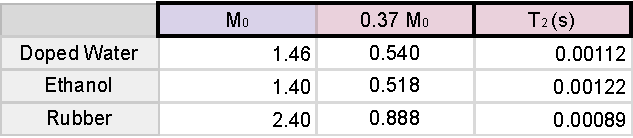
\includegraphics[scale = 0.78]{./images/B2_slopes_estimate-crop}
        \caption{Estimate of $T_2^*$ using the initial magnetization}
        \label{tab:B2_FID_log_best_fit_table_estimate}
    \end{table}
\end{itemize}

\newpage

\section{Conclusion}\label{sec:conclusion}
% Your conclusion content goes here.

\end{document}
